%!TEX root = main.tex
\chapter{研究现状分析}
\label{ch:研究现状分析}

\section{异构高性能计算发展现状}
% 神威·太湖之光
高性能计算机的研究与应用水平是一个国家综合国力和科技创新能力的重要标志之一,我国大力推进研制具有高性能、高可靠性的超级计算机。2010年,天河-1A\cite{yang2011tianhe}超级计算机以峰值性能4.7 Pflops、持续性能2.5 Pflops,超越美洲虎(Jaguar)超级计算机成为我国第一台世界上最快的超级计算机。2013年,位于广州超级计算中心的天河二号超级计算机\cite{liao2014milkyway}以54.9 Pflops的峰值性能、33.8 Pflops的持续性能再次超越美国泰坦(Titan)超级计算机成为世界上最快的超级计算机,并连续 6 次摘得世界超级计算机排名榜单 TOP500 的桂冠。2016年,国家并行计算机工程技术研究中心研制,安装在国家超级计算无锡中心的神威·太湖之光\cite{fu2016sunway}超级计算机以峰值性能125 Pflops、持续性能93 Pflops超越天河二号登顶TOP500榜单之首,并截止至2017年11月已连续四次排名第一。自2010年以来,我国超级计算机的峰值性能从天河-1A的4.7 Pflops迅猛提升到神威·太湖之光的125 Pflops,共11次问鼎TOP500榜首,标志着我国已经成为了世界超算大国。

超算的性能在持续提升,传统提升计算能力的方式有两种——提升CPU时钟频率和增加计算核心数量,这两种方式遇到了散热和功耗瓶颈。近年来越来越多的高性能计算平台采用异构计算架构\cite{buyya1999high}。异构计算架构由不同指令集和体系结构的计算单元组成,通常以CPU为核心控制单元,异构加速器为主要计算器件,通过PCIe与主板连接并进行数据传输。与CPU相比,异构加速器主频较低,但具有更多的核心数、更高并行计算能力和能耗比\cite{hong2010integrated}。主流的异构计算平台包括CPU+GPU、CPU+Xeon Phi以及CPU+FPGA。

目前应用最广泛的异构加速器是NVIDIA公司推出的面向通用计算的图形处理器\cite{nvidia2008programming}(GPU)。在最新(2017年11月)的TOP500榜单的前100台超算中,共有19台超算采用了NVIDIA GPU加速器,其中包括我国的天河-1A超级计算机,配备了7,168块Tesla M2050计算卡;瑞士的“Piz Daint”超级计算机\cite{PIZDAINT},配备了5,272块NVIDIA最新的P100加速卡;美国的Titan超级计算机\cite{shimpi2012inside},配备了18,688块Tesla K20X加速卡。

另外一个应用较为广泛的是由英特尔公司推出的Xeon Phi协处理器\cite{jeffers2013intel}。GPU虽有数以千计的运算核心,但编程门槛较高,通常需要使用CUDA\cite{cook2012cuda}重写CPU代码。Xeon Phi浮点运算性能强,同时编程门槛较低,可复用CPU代码,因此也受到了许多异构超算的青睐,如排名世界第二的天河二号超级计算机,配备了48,000块Xeon Phi\cite{liao2014milkyway};排名世界第七的Trinity超级计算机\cite{Trinity},采用Cray XC40和Xeon Phi 7250,共有979,968核心;排名第八的Cori超级计算机\cite{doerfler2018evaluating},配备了9,688块Xeon Phi 7250。

基于GPU和Xeon Phi的高性能异构计算平台在许多科学应用中发挥出强大的计算力。例如薛巍将基于欧拉方程的大气模式在天河二号超级计算机的6144个异构计算节点进行优化,取得1.74 Pflops的双精度浮点计算性能\cite{xue2015ultra}。Heinecke将地震灾害模拟扩展到了天河二号超级计算机的8,192个异构计算机节点,并取得了8.6 Pflops的峰值性能\cite{heinecke2014petascale}。Jeroen使用“泰坦”超级计算机的18,600个GPU节点进行银河系天体模拟,取得了24.77 Pflops的计算性能\cite{bedorf201424}。此外,GPU和Xeon Phi异构高性能计算还支持诸如生物医药\cite{tumeo2010accelerating,chen2008gpu}、航空航天\cite{habib2012universe,kampolis2010cfd}、军事科技\cite{ariga2014fast,fronckowiak2009using}等多个应用领域,均取得了突出的成果。

GPU和Xeon Phi异构加速器虽然具有浮点运算能力强,计算吞吐量高等优点,但并不适用于低延迟、低功耗等应用场景。现场可编程逻辑阵列(field-programmable gate array, FPGA)具备低延迟、低功耗、可编程等优点,适用于加密算法\cite{elbirt2000fpga,elbirt2000fpga,hauser1997garp}、金融分析\cite{zhang2005reconfigurable,jin2013optimising,tse2010reconfigurable,becker2015maxeler}、机器学习\cite{irick2008hardware,zhang2015optimizing,wang2017dlau}等等领域。例如本文作者使用FPGA平台加速了高斯混合模型期望值最大化(EM-GMM)算法,取得了比Titan-X GPU高出39倍的性能\cite{he2017fully}。在金融相关的工作中,本文作者为上海金融期货交易所设计了基于FPGA硬件平台的低延迟行情服务器\cite{fu2017nanosecond,he2017exploring,fu2017accelerating},最低延迟可达$3\mu s$。但是,由于FPGA开发难度高、通用性低、浮点运算能力较弱,并未进入TOP500榜单,但Amazon、阿里巴巴、腾讯、百度等公司为不同企业提供了丰富的FPGA云服务\cite{tarafdar2018designing}。

高性能计算平台性能的提升一方面通过升级硬件,另一方面依赖于增加节点或加速器数量。然而超级计算机大规模、长时间的运行需要耗费大量电量\cite{reed2015exascale}。片上异构的处理器将任务调度单元和异构计算单元集成到同一片芯片上,有利于数据共享和降低功耗,很好地缓解了超算功耗大的问题。目前TOP500榜首的神威·太湖之光超级计算机正是基于片上异构众核处理器\cite{fu2016sunway}——申威26010处理器(SW26010),每个申威26010处理器具有260个核心,峰值性能为3 Tflops,与NVIDIA K80 GPU、Intel Knight Landing性能相当\cite{einkemmer2017evaluation,sodani2016knights}。神威·太湖之光超级计算机相对于其他超算在能耗上有很大的提升,性能功耗比为$6.05Gflops/W$,是排名第二的天河二号超级计算机的3倍。从2016年发布以来,神威·太湖之光超级计算机已经在多个领域为大型科学应用提供了助力,如地震模拟\cite{fu201718}、机器学习\cite{fang2017swdnn}、气候模式\cite{yang201610m,fu2016refactoring}、海洋模拟\cite{qiao2016highly}、材料科学\cite{zhang2016extreme}等等。其中“7.9 Pflops的大气模式的全隐式动力框架求解器”和“18.9 Pflops的非线性唐山大地震模拟”都在神威·太湖之光超级计算机上扩展到千万核心,分别获得了2016年和2017年高性能计算应用领域最高奖——“戈登·贝尔”奖。

综上调研可知,片上异构高性能计算平台在计算效率、集成度、能耗比等方面给大规模科学计算提供了巨大的空间,是未来异构高性能计算研究的新兴方向。

\section{面向天然大地震的高性能计算研究}

天然大地震模拟作为高性能计算应用中典型的“巨大挑战”之一,一直以来都是超级计算机的主要服务对象。大规模地震模拟的研究工作可以追溯到1996年,Bielak等人在Cray T3D的256个处理器上使用非结构化网格进行了区域大小为140km $\times$ 100km $\times$ 20km的地震模拟\citep{bao1996earthquake},性能达到了8 Tflops,这是最早的地震数值模拟工作之一。

从地震发生概率角度出发,多数大规模地震模拟工作都集中在日本和美国湾区等地震活跃地区。例如,美国加州理工学院和日本JAMSTEC合作的地震模拟工作在2003年第一次获得了“戈登·贝尔”奖\citep{es-gb-2003}。这个工作使用谱元法\cite{chen2006glueball}将模拟区域划分成平均网格间距为2.9km的立方体,在地球模拟器上使用了1,944个处理器进行了全球地震波模拟,取得了5 Tflops的峰值性能。这项工作随后经过扩展开发成为著名的SPECFEM3D\_GLOBE软件\cite{bozdag2010specfem3d_globe},并随着新一代超级计算机的发展不断演变。

2008年,Carrington等人使用SPECFEM3D\_GLOBE软件在Ranger超级计算机上使用32,000个计算核心进行地震模拟\cite{carrington2008high},模拟的网格分辨率提高到了800m、频率达到0.5Hz、峰值性能达到了28.7Tflops。同年,Carrington等人又在Jaguar超级计算机上使用了29,000个计算核心进行地震模拟,由于Jaguar超级计算机内存带宽较高,该模拟取得了35.7 Tflops的峰值性能。2012年,SPECFEM3D\_GLOBE的代码经过升级使之能够支持GPU异构平台。Rietmann等人将地震波传播模拟扩展到了896个CPU-GPU节点\citep{rietmann2012forward},性能达到了35 Tflops。

另一种能够支持大规模地震模拟的数值方法是SeisSol软件中的任意高阶导数不连续Galerkin有限元方法\cite{godel2010scalability}(DG-FEM)。SeisSol在天河二号超级计算机的8,192个节点上模拟了1992年Landers M7.2地震\citep{tianhe2-2014gb},该模拟包含了1.91亿个四面体元素和960亿个自由度,持续性能达到了8.6 Pflops。

与其他方法相比,SeisSol中的DG-FEM算法将数值问题转化为计算受限的稠密矩阵运算,充分发挥了Intel Xeon Phi加速器的计算性能。然而,高阶数值方法也增加了计算和内存的复杂性,进一步限制了可解问题的最大尺寸和计算时间。2017年,Breuer等人使用DG-FEM方法在Cori-II超级计算机的612,000个核心上进行了超大规模融合地震模拟\citep{breuer2017edge},峰值性能达到了10.4 Pflops。

近期,也有学者使用隐式有限元求解器\cite{geradin1983implicit}在日本“京”超级计算机\cite{yokokawa2011k}上探索地震模拟的潜力。T. Ichimura等人提出了基于MPI-OpenMP的三维混合地震波放大模拟软件——GAMERA \citep {ichimura2014physics}和GOJIRA \citep {ichimura2015implicit}。GOJIRA以29.7秒的时间步长求解了超过1万亿次自由度的地震模拟。利用日本“京”超级计算机的全部663,552个CPU核心,该求解器的峰值性能达到了1.97 Pflops。然而,这两项工作主要集中在城市中的建筑物(通常大小为几十公里)和地震波放大模拟的场景上,他们并不能在数百公里范围内进行大规模的地震模拟。

作为世界领先的地震研究联盟,也是世界上最大的跨学科、跨国家的地球科学合作机构,南加州地震中心(SCEC)在地震模拟领域取得了重大的进展。SCEC在2004年启动了TeraShake项目,该项目从美国科学基金(NSF)资助的TeraGrid超级计算机\citep{teragrid}的2,048个处理器起步,逐步将地震模拟的规模扩展到具有40,000个核心的BlueGene超算\cite{adiga2002overview}。
TeraShake项目发现南圣安德烈亚斯断层的破裂指向性是一个震源效应,它可能与沉积盆地的场地效应耦合,大大增加了洛杉矶的地震危险性。该项目有效地展示了大规模地震模拟的科学效益。

该项目的另一个重要成果是AWP-ODC\cite{awpodc}(Anelastic Wave Propagation by Olsen, Day and Cui)开源软件,该软件在不同的地震研究项目中被广泛使用。2010年,AWP-ODC能够支持千万亿次超级计算机上的大规模地震模拟\citep{cui2010scalable}。Yifeng Cui等人使用Jaguar超级计算机的223,074个计算核心模拟了南加州地震,模拟区域为810km $\times$ 405km $\times$ 85km,空间分辨率为40m,最大频率为2Hz,持续性能达到了220 Tflops。

2013年,AWP-ODC经过扩展得以支持GPU异构平台。Yifeng Cui等人使用了Titan超级计算机的16,384个GPU解决了规模为20,480 $\times$ 20,480$\times$2,048个网格点的地震模拟问题,并取得了2.33 Pflops的持续性能。

2016年,SCEC进一步完善AWP-ODC软件,使其支持非线性效应的地震模拟,这是高频地震模拟中一大关键。R.Daniel等人使用了Titan超级计算机半机资源进行了非线性地震模拟\citep{roten2016high},性能达到了1.6 Pflops。

表\ref{tb:rw-comp}总结了已有的大规模地震模拟工作。在大约二十年的时间里,支持地震模拟的超级计算机从256个处理器发展到如今1000万个计算核心,地震模拟的规模也从数百万个元素扩展到数十亿个元素,占用内存空间从GB量级扩展到了PB量级,地震模拟性能也从8 Gflops提高到15 Pflops。

\begin{landscape}
\begin{table*}[ht]
\caption{基于超级计算机的大规模地震模拟已有工作总结。这些数字是从已发表的论文中获得的。未报告的值被标记为“-”。对于数值方法,FD指的是有限差分法,SEM指的是谱元法,DG-FEM指不连续的Galerkin有限元法。}
\label{tb:rw-comp}
\centering
\resizebox{1.55\textwidth}{!}{%
\begin{tabular}{ccccccccccc}
\hline\hline
\multicolumn{2}{c}{工作} & 时间 & 平台 & 架构 & 规模 & 网格点数 & 自由度 & 性能 & 内存 & 数值方法 \\ \hline\hline
EGMM & \cite{bao1996earthquake} & 1996 & Cray T3D & Alpha CPU & 256 CPU & 1340万 & 4020万 & 8 Gflops & 16 GB & FD \\ \hline\hline
\multirow{4}{*}{SPECFEM3D} & \citep{es-gb-2003} & 2003 & 地球模拟器 & NEC SX-6 & 1,944 CPU & 55亿 & 146亿 & 5 Tflops & 2.5 TB & SEM \\ \cline{2-11}
 & \multirow{2}{*}{\citep{carrington2008high}} & 2008 & Ranger & 4核Opteron & 32,000核 & -- & -- & 28.7 Tflops & -- & SEM \\
 & & 2008 & Jaguar & 4核Opteron & 29,000核 & -- & -- & 35.7 Tflops & -- & SEM \\ \cline{2-11}
 & \citep{rietmann2012forward} & 2012 & Cray XK6 & Nvidia Fermi & 896 GPUs & 80亿 & 220亿 & 135 Tflops & 3.5 T & SEM \\ \hline\hline
\multirow{2}{*}{SeiSol} & \multirow{2}{*}{\citep{tianhe2-2014gb}} & \multirow{2}{*}{2014} & \multirow{2}{*}{Tianhe-2} & 12核Xeon + & 196,608核 & 1.91亿 & \multirow{2}{*}{960亿} & \multirow{2}{*}{8.6 Pflops} & \multirow{2}{*}{--} & \multirow{2}{*}{DG-FEM} \\
 & & & & 59核Xeon Phi & 1,400,832核 & 四面体 & & & & \\ \cline{2-11}
\multirow{2}{*}{EDGE} & \multirow{2}{*}{\citep{breuer2017edge}} & \multirow{2}{*}{2017} & \multirow{2}{*}{Cori-II} & \multirow{2}{*}{68核Xeon Phi} & \multirow{2}{*}{612,000核} & 3.41亿 & \multirow{2}{*}{--} & \multirow{2}{*}{10.4 Pflops} & \multirow{2}{*}{32 TB} & \multirow{2}{*}{DG-FEM} \\
 & & & & & & 四面体 & & & & \\ \hline\hline
GAMERA & \citep{ichimura2014physics} & 2014 & K Computer & 8核SPARC64 & 663,552核 & -- & 270亿 & 0.804 Pflops & -- & 隐式FEM \\ \cline{2-11}
GOJIRA & \citep{ichimura2015implicit} & 2015 & K Computer & 8核SPARC64 & 663,552核 & 2700亿 & 1.08万亿 & 1.97 Pflops & -- & 隐式FEM \\ \hline\hline
\multirow{6}{*}{AWP-ODC} & \multirow{2}{*}{\citep{cui2010scalable}} & \multirow{2}{*}{2010} & \multirow{2}{*}{Jaguar} & \multirow{2}{*}{6核Istanbul} & \multirow{2}{*}{223,074核} & \multirow{2}{*}{4360亿} & \multirow{2}{*}{1.31万亿} & \multirow{2}{*}{220 Tflops} & \multirow{2}{*}{127 TB} & FD \\
 & & & & & & & & & & 线性 \\ \cline{2-11}
 & \multirow{2}{*}{\citep{cui2013physics}} & \multirow{2}{*}{2013} & \multirow{2}{*}{Titan} & 16核Opteron + & 229,376 SMXs & \multirow{2}{*}{8590亿} & \multirow{2}{*}{2.58万亿} & \multirow{2}{*}{2.33 Pflops} & \multirow{2}{*}{250TB} & FD \\
 & & & & Nvidia K20x & 16,384 GPUs & & & & & 线性 \\ \cline{2-11}
 & \multirow{2}{*}{\citep{roten2016high}} & \multirow{2}{*}{2016} & \multirow{2}{*}{Titan} & 16核Opteron + & 114,688 SMXs & \multirow{2}{*}{3290亿} & \multirow{2}{*}{9870亿} & \multirow{2}{*}{1.6 Pflops} & \multirow{2}{*}{129TB} & FD \\
 & & & & Nvidia K20x & 8,192 GPUs & & & & & 非线性 \\ \hline\hline
\multirow{4}{*}{本文工作} & \multirow{2}{*}{无压缩} & \multirow{2}{*}{2017} & \multirow{2}{*}{太湖之光} & 260核 & \multirow{2}{*}{1,014,000核} & \multirow{2}{*}{3.99万亿} & \multirow{2}{*}{11.9万亿} & \multirow{2}{*}{15.2 Pflops} & \multirow{2}{*}{892 TB} & FD \\
 & & & & SW26010 & & & & & & 线性 \\ \cline{2-11}
 & \multirow{2}{*}{含压缩} & \multirow{2}{*}{2017} & \multirow{2}{*}{太湖之光} & 260核 & \multirow{2}{*}{1,014,000核} & \multirow{2}{*}{7.8万亿} & \multirow{2}{*}{23.4万亿} & \multirow{2}{*}{18.9Pflops} & \multirow{2}{*}{724TB} & FD \\
 & & & & SW26010 & & & & & & 非线性 \\\hline\hline
\end{tabular}
}
\end{table*}
\end{landscape}


此外,不同的软件包采用不同的数值方法(如SPECFEM3D的SEM、SeisSol和EDGE的DG-FEM、GAMERA和GOJIRA的隐式有限元、AWP-ODC的有限差分),因此不可能用一个衡量标准对他们进行统一比较。一般而言,基于有限元的方法具有更好的地形处理能力,可以用少量的网格模拟复杂的场景,但是对于非线性问题的收敛性可能会面临严重的效率问题。相比之下,有限差分(FD)具有计算规整、内存访问和节点间通信友好等优点,但对计算和存储容量的需求很高,这一度被认为是不切实际的解决方案。近些年来,随着超算的发展,有限差分方法被普遍认为更适合大规模并行计算。

综上考虑所有主流的地震模拟软件,AWP-ODC在过去的几十年里累积了大量SCEC在地球物理和计算机领域的工作,提供了最先进的功能,支持塑性和非弹性衰减物理特性,且能够在半天内完成大规模的地震模拟。

因此,本文工作以AWP-ODC为原型,根据神威·太湖之光独特的硬件架构进行了重新设计并进行深度优化,将神威超算的计算、内存容量、内存带宽、IO带宽和通信带宽等资源都发挥到了极致。本文工作的地震模拟性能从Titan超级计算机的2.3 Pflops提高到神威·太湖之光的15.2 Pflops,模拟的规模比原来大4-5倍。此外,本文工作还提出了基于异构众核架构的实时压缩方案,将地震模拟的性能进一步提升到了18.9 Pflops,支持的最大频率和最高分辨率分别提升到了18Hz和8m。与2013年和2016年在Titan超级计算机上的AWP工作相比,本文工作将地震仿真性能提高了9倍,最大的可解问题尺寸提高了9倍到10倍。



\section{面向地球物探反演成像的高性能计算研究}

%自上个世纪70年代初至今,波动方程偏移经历了发展-停滞-再发展的阶段。到了20世纪90年代,随着计算技术的飞跃发展,以及克希霍夫叠前深度偏移技术在墨西哥湾的成功应用,再次把偏移技术推向了发展高峰。进入21世纪,波动方程叠前深度偏移技术得到了较快的发展,并借助于高性能集群计算技术的发展在实际生产中得到了广泛的应用[2]。

地球物探由于具备巨大的商业推动,是高性能计算最重要的应用之一。自上个世纪90年代末以来,人工地震勘探的偏移和成像算法的应用在高性能计算的推动下取得了巨大的进展,对计算、内存、IO的需求也呈指数级增长。以Kirchhoff三维叠前深度偏移\cite{yilmaz2001seismic}的计算量为参考标准,共方位角波动方程偏移\cite{rickett2002offset}在精度和分辨率上比Kirchhoff方法更有优势,其计算量约为后者的2倍;共炮域波动方程叠前深度偏移\cite{zhang2005theory}在复杂构造地区的成像效果要好于Kirchhoff叠前深度偏移,但其计算量约为后者的10倍。2003年,Y. Sun等人提出射线偏移算法\cite{sun20003}对道集以组的形式进行处理,极大的降低了计算需求。2010年左右,由于高性能计算机的迅猛发展,基于声波的逆时偏移算法\cite{baysal1983reverse}能以更高分辨率、更精确的成像效果备受学术界和工业界的青睐,其计算量约为传统Kirchhoff算法的100倍。近些年来,全波形反演算法\cite{tarantola1984inversion}以其理论的完备性成为研究热点。图\ref{fig:seismicmethod}展示了近20年来人工地震勘探算法对运算速度需求的变化趋势。

\begin{figure}[ht]
\centering
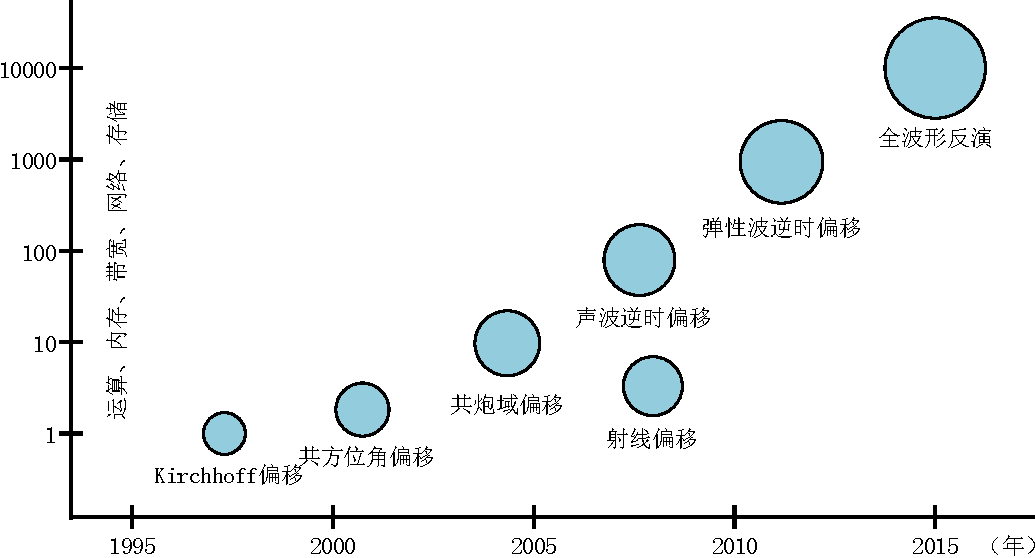
\includegraphics[width=0.7\columnwidth]{地震勘探算法与资源需求-crop.pdf}
\caption{人工地震勘探算法对运算资源需求的变化趋势。}
\label{fig:seismicmethod}
\end{figure}

地震波正演、逆时偏移、全波形反演等地球物理勘探算法的核心计算是使用显式的有限差分算法更新地震波波场。近些年来,有一系列基于GPU、Xeon Phi和FPGA异构高性能平台的有限差分算法或$Stencil$加速工作,并取得了非常理想的性能结果\cite{qawasmeh2015gpu,martinez2015towards,fang2015optimizing,liu20153d,clapp2015seismic,costa2015half,fu2012revisiting,clapp2010selecting}。例如,J.Fang等人在GPU平台对复杂$Stencil$计算进行优化,相比于12核CPU取得了9.6倍的性能提升\cite{fang2015optimizing}。A. Qawasmeh等人在GPU平台上使用OpenACC工具移植和优化基于波场方程的逆时偏移算法,取得了比CPU快10倍的性能提升\cite{qawasmeh2015gpu}。Y. Yang等人在Xeon Phi平台优化了三维弹性波正演方法,取得了相对于12核CPU 3.7倍的性能提升\cite{you2013accelerating}。H. Fu等人在FPGA平台上优化了逆时偏移算法,取得了与72核CPU相当的性能,并获得了10倍的能耗比提升。

全波形反演方法(full waveform inversion; FWI)于1984年由Tarantola提出,能准确地从人工地震记录中提取大量地下介质信息\cite{tarantola1984inversion,plessix2012full,brossier2009seismic}。该方法通过对比数值模拟合成的地震记录和实际观测的人工地震记录误差,迭代更新模型参数,从而反演地下介质模型\cite{yushu}。然而,由于该方法伴随着巨大的计算开销,直到2010年超级计算机和NVIDIA GPU,Intel Xeon Phi等加速器为全波形反演方法提供了足够的计算能力,该方法才逐渐成为研究热点,并为各大石油公司采用。

尽管全波形反演方法在理论上能够很好地反演地下介质模型,但在实际生产中却面临着两大问题。一方面,全波形反演方法需要非常准确的初始速度模型作为输入,否则该算法很容易陷入局部最优\cite{virieux2009overview}。虽然地震记录中的低频信号成分能够降低对初始速度模型的要求,但是在实际生产场景中往往很难捕捉到低频信号\cite{sirgue2006importance}。另一方面全波形反演方法对地震记录数据中的噪音非常敏感,这严重影响了该算法的实际成像效果。

本文工作在传统完全反演\cite{tarantola1982generalized}(total inversion)的基础上,通过使用集合卡尔曼滤波\cite{evensen2003ensemble}中的集合协方差来近似完全反演中的协方差算子,提出了集合全波形反演方法(EnFWI)\cite{yushu,he2015ensemble}。集合全波形反演方法有效降低了在完全反演中更新协方差算子的计算开销,使之可以在一般的分布式集群中进行计算。然而,由于速度模型中需要更新的参数数量比集合样本数量大2-4个数量级,集合卡尔曼滤波的更新增量受到很大的限制。对此,集合全波形反演方法再次引入了震源编码技术\cite{krebs2009fast}。震源编码技术将所有的震源和地震记录分别进行叠加,每次叠加时不同的震源和地震记录分别使用不同的震源编码,在有利于克服局部收敛的同时\cite{castellanos2014fast},克服了集合卡尔曼滤波低秩空间的局限性,也显著地提升了计算性能。

\section{本章小结}

本章首先介绍了世界领先的超级计算机,异构计算架构已经逐渐成为超级计算机的主流架构,并为不同领域的科学应用提供丰富的计算能力。神威·太湖之光超级计算机以高运算效率、高能耗比大幅领先排名第二的超级计算机,基于片上异构架构的超级计算机有望成为未来E级计算的主流架构。天然地震模拟和人工地震勘探算法都对高性能计算提出了巨大的需求和挑战,研究面向神威·太湖之光超级计算机的地震模拟并行优化方法具有重要的意义。
